\documentclass[xcolor=dvipsnames,table]{beamer} % dvipsnames gives more built-in colors
\usepackage[utf8]{inputenc}
\usepackage[english]{babel}
\usepackage{xcolor}
\usepackage{listings}
\usepackage{caption}
\usepackage{subcaption}
\usepackage{multicol}
\usepackage{xcolor}
\usepackage{pbox}

%%%%%%%%%%%%%%%%%%%%%%%%%%%%%%%%%%%%%%%%%%%%%%%%%%%%%%%%%%%%%%%%%%%%%%%%%%%%%%%%%%%%%%%%%%%%%%%%%%%%%%%%%%%%%%%%%%%%%%%%
%%%%%%%%%%%%%%%%%%%%%%%%%%%%%%%%%%%%%%%%%%%%%% CONFIGURACIONES %%%%%%%%%%%%%%%%%%%%%%%%%%%%%%%%%%%%%%%%%%%%%%%%%%%%%%%%%
%%%%%%%%%%%%%%%%%%%%%%%%%%%%%%%%%%%%%%%%%%%%%%%%%%%%%%%%%%%%%%%%%%%%%%%%%%%%%%%%%%%%%%%%%%%%%%%%%%%%%%%%%%%%%%%%%%%%%%%%

\usetheme{Madrid}
\useoutertheme{miniframes} % Alternatively: miniframes, infolines, split
\useinnertheme{circles}

\definecolor{UBCblue}{rgb}{0.04706, 0.13725, 0.26667} % UBC Blue (primary)
\definecolor{blueapi}{rgb}{0.74, 0.83, 0.9}
\newcommand{\si}{
\includegraphics[height=0.3cm]{../figures/ok-icon.png}}
\newcommand{\no}{
\includegraphics[height=0.3cm]{../figures/x-icon.jpg}}

\lstset{ %
  backgroundcolor=\color{white}, 
  basicstyle=\footnotesize,       
  breakatwhitespace=false,        
  breaklines=true,                 
  captionpos=b,                    
  commentstyle=\color{green},   
  escapeinside={\%*}{*)},        
  extendedchars=true,              
  frame=single,                  
  keywordstyle=\color{blue},       
  language=Prolog,                
  numbers=left,                    
  numbersep=5pt,                   
  numberstyle=\tiny\color{gray},
  rulecolor=\color{black},        
  showspaces=false,               
  showstringspaces=false,          
  showtabs=false,                  
  stepnumber=2,                    
  stringstyle=\color{BrickRed},   
  tabsize=2,                      
  title=\lstname,                  
  morekeywords={not,\},\{,preconditions,effects },            
  deletekeywords={time}            
}

\usecolortheme[named=UBCblue]{structure}
%\usecolortheme[named=Mahogany]{structure} % Sample dvipsnames color

\title[VirtShell]{\textbf{VirtShell} \\ Framework para aprovisionamiento de soluciones virtuales}
\date{\tiny\today}
\titlegraphic{
\includegraphics[width=0.9cm]{logo_univalle.pdf}}
\author[CALlanoR]{\textbf{Carlos Alberto Llano R.}}
\institute[www.univalle.edu.co]{Escuela de Ingeniería de Sistemas y Computación \\ Maestría en Ingeniería con énfasis en Ingeniería de Sistemas y Computación \vspace{0.2cm} \\ Director: \\ \textbf{John Alexander Sanabria}}

\begin{document}

%%%%%%%%%%%%%%%%%%%%%%%%%%%%%%%%%%%%%%%%%%%%%%%%%%%%%%%%%%%%%%%%%%%%%%%%%%%%%%%%%%%%%%%%%%%%%%%%%%%%%%%%%%%%%%%%%%%%%%%%
%%%%%%%%%%%%%%%%%%%%%%%%%%%%%%%%%%%%%%%%%%%%%%%%%%%%% TITULO %%%%%%%%%%%%%%%%%%%%%%%%%%%%%%%%%%%%%%%%%%%%%%%%%%%%%%%%%%%
%%%%%%%%%%%%%%%%%%%%%%%%%%%%%%%%%%%%%%%%%%%%%%%%%%%%%%%%%%%%%%%%%%%%%%%%%%%%%%%%%%%%%%%%%%%%%%%%%%%%%%%%%%%%%%%%%%%%%%%%

\frame{\titlepage}

\setcounter{tocdepth}{1}  % Esto permite esconder las subsections
\frame{\frametitle{Contents}\tableofcontents}

\logo{\hspace*{0.6\textwidth}
\includegraphics[width=0.6cm]{logo_univalle}\hspace*{0.3cm}}

%%%%%%%%%%%%%%%%%%%%%%%%%%%%%%%%%%%%%%%%%%%%%%%%%%%%%%%%%%%%%%%%%%%%%%%%%%%%%%%%%%%%%%%%%%%%%%%%%%%%%%%%%%%%%%%%%%%%%%%%
%%%%%%%%%%%%%%%%%%%%%%%%%%%%%%%%%%%%%%%%%%%%%%%%%%% OBJETIVOS %%%%%%%%%%%%%%%%%%%%%%%%%%%%%%%%%%%%%%%%%%%%%%%%%%%%%%%%%%
%%%%%%%%%%%%%%%%%%%%%%%%%%%%%%%%%%%%%%%%%%%%%%%%%%%%%%%%%%%%%%%%%%%%%%%%%%%%%%%%%%%%%%%%%%%%%%%%%%%%%%%%%%%%%%%%%%%%%%%%

\section{Propósitos alcanzados}

\frame{ \frametitle{Objetivos}
	\setbeamercolor{block title}{fg=white,bg=blue!75!black}
	\begin{block}{General}
	Diseñar un framework web, que permita el aprovisionamiento de software automático, para ambientes virtualizados.
	\end{block}
	\pause
	\vspace{0.3cm}
	\setbeamercolor{block title}{fg=white,bg=blue!75!black}
	\begin{block}{Específicos}
		\begin{enumerate}
			\item Evaluar diferentes técnicas y soluciones de aprovisionamiento que se utilizan en la actualidad.
			\item Evaluar diferentes mecanismos de aprovisionamiento.
			\item Realizar una ejemplificación del framework.
		\end{enumerate}
	\end{block}
}

%%%%%%%%%%%%%%%%%%%%%%%%%%%%%%%%%%%%%%%%%%%%%%%%%%%%%%%%%%%%%%%%%%%%%%%%%%%%%%%%%%%%%%%%%%%%%%%%%%%%%%%%%%%%%%%%%%%%%%%%
%%%%%%%%%%%%%%%%%%%%%%%%%%%%%%%%%%%%%%%%%%%%%%%%% OBJETIVO #1 %%%%%%%%%%%%%%%%%%%%%%%%%%%%%%%%%%%%%%%%%%%%%%%%%%%%%%%%%%
%%%%%%%%%%%%%%%%%%%%%%%%%%%%%%%%%%%%%%%%%%%%%%%%%%%%%%%%%%%%%%%%%%%%%%%%%%%%%%%%%%%%%%%%%%%%%%%%%%%%%%%%%%%%%%%%%%%%%%%%

\subsection{Técnicas y soluciones de aprovisionamiento actuales (Objetivo \#1)}

\frame{ \frametitle{Técnicas de Virtualización trabajadas}
	\begin{figure}
		\captionsetup[subfigure]{labelformat=empty}
		\begin{subfigure}{.5\textwidth}
			\centering
			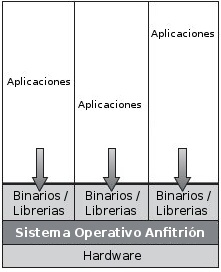
\includegraphics[height=5cm]{../../architecture/v1/diagrams/contenedores.jpg}
			\caption{Contenedores}
		\end{subfigure}%
		\pause
		\begin{subfigure}{.5\textwidth}
			\centering
			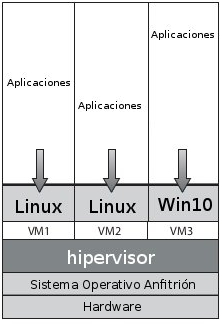
\includegraphics[height=5cm]{../../architecture/v1/diagrams/virtualmachine.jpg}
			\caption{Máquinas Virtuales}
		\end{subfigure}%
	\end{figure}
}

\frame{ \frametitle{Soluciones de aprovisionamiento evaluadas}
\begin{multicols}{2}
	\begin{itemize}
		\item Fabric
		\item Chef
		\item Puppet
		\item Juju
		\item CFEngine
		\item Bcfg2
		\item Ansible
		\item Cobbler
		\item SmartFrog
		\item Amazon EC2
		\item Docker composer
		\item SaltStack
		\item Vagrant
	\end{itemize}
\end{multicols}
}

\frame{ \frametitle{Soluciones de aprovisionamiento evaluadas}
\scriptsize
\begin{tabular}{| l | l | l | l | l | l | l |}
	\hline
	\rowcolor{blueapi}
	\textbf{Solución} & \textbf{Sop.Nubes} & \textbf{Curv.Apren} & \textbf{Crea} & \textbf{Aprov} & \textbf{API REST} & \textbf{Mult.SO} \\ [0.5ex]
	\hline\hline
	Chef          & Todas                           & Alta     & \si     & \si   & \si   & \si   \\ \hline
	Juju          & \pbox{5cm}{OpenStack \\ MAAS}   & Baja     & \si     & \si   & \no   & \no   \\ \hline
	Puppet        & La mayoria                      & Media    & \no     & \si   & \no   & \si   \\ \hline
	Ansible       & \pbox{5cm}{Amazon \\ OpenStack} & Baja     & \no     & \si   & \no   & \si   \\ \hline
	Amazon EC2    & Amazon                          & Media    & \si     & \si   & \si   & \si   \\ \hline
	Docker        & \no                             & Media    & \si     & \si   & \si   & \si   \\ \hline
	Vagrant       & \no                             & Baja     & \si     & \si   & \no   & \si   \\ \hline
\end{tabular}
}

%%%%%%%%%%%%%%%%%%%%%%%%%%%%%%%%%%%%%%%%%%%%%%%%%%%%%%%%%%%%%%%%%%%%%%%%%%%%%%%%%%%%%%%%%%%%%%%%%%%%%%%%%%%%%%%%%%%%%%%%
%%%%%%%%%%%%%%%%%%%%%%%%%%%%%%%%%%%%%%%%%%%%%%%%% OBJETIVO #2 %%%%%%%%%%%%%%%%%%%%%%%%%%%%%%%%%%%%%%%%%%%%%%%%%%%%%%%%%%
%%%%%%%%%%%%%%%%%%%%%%%%%%%%%%%%%%%%%%%%%%%%%%%%%%%%%%%%%%%%%%%%%%%%%%%%%%%%%%%%%%%%%%%%%%%%%%%%%%%%%%%%%%%%%%%%%%%%%%%%

\subsection{Evaluar diferentes mecanismos de aprovisionamiento. (Objetivo \#2)}

\frame{ \frametitle{Selección del mecanismo de aprovisionamiento}
	\setbeamercolor{block title}{fg=white,bg=blue!75!black}
	\begin{block}{Se evaluaron diferentes formas de escritura de scripts de aprovisionamiento}
		\begin{itemize}
			\item json
			\item xml
			\item yaml
			\item archivos texto 
			\item lenguajes de programación (ruby, python, etc.)
			\item bash
		\end{itemize}
	\end{block}	
}

\frame{ \frametitle{Selección del mecanismo de aprovisionamiento}
	
\includegraphics[height=5cm]{../figures/and-the-winner-is.jpg}
	\pause
	
\includegraphics[height=5cm]{../figures/bin-bash.png}
}

\frame{ \frametitle{Selección del mecanismo de aprovisionamiento}
	\begin{center}
		
\includegraphics[height=3cm]{../figures/bash_on_windows.png}
	\end{center}
}

\frame{ \frametitle{Selección del mecanismo de aprovisionamiento}
	\setbeamercolor{block title}{fg=white,bg=blue!75!black}
	\begin{block}{Se evaluaron diferentes formas de guardar los scripts en el sistema}
		\begin{itemize}
			\item repositorio central propio?
			\item enviarlo en el momento del aprovisionamiento?
		\end{itemize}
	\end{block}
}

\frame{ \frametitle{Selección del mecanismo de aprovisionamiento}
	\setbeamercolor{block title}{fg=white,bg=blue!75!black}
	\begin{block}{Solución}
		\begin{center}
			
\includegraphics[height=2cm]{../figures/git---github-logo.jpg}
		\end{center}
	\end{block}
}

\frame{ \frametitle{Evaluación y selección de un estilo arquitectural}
	\begin{center}
		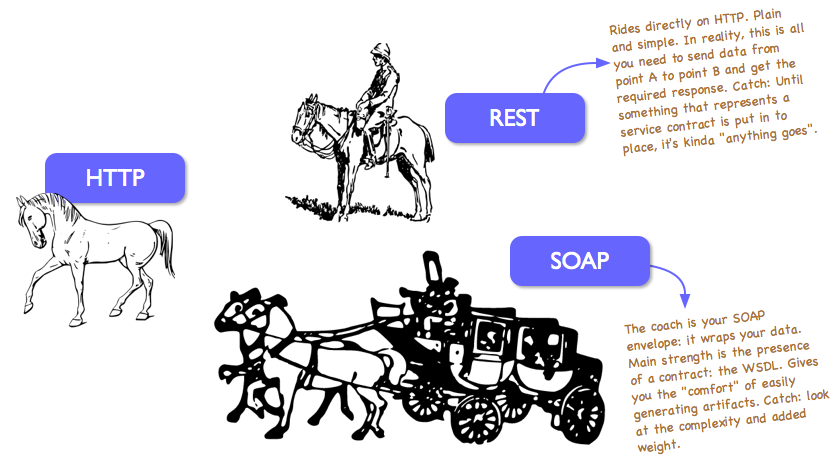
\includegraphics[height=5.5cm]{../figures/restvssoap1.png}
	\end{center}
}

\frame{ \frametitle{Evaluación y selección de un estilo arquitectural}
	\begin{figure}
		\centering
		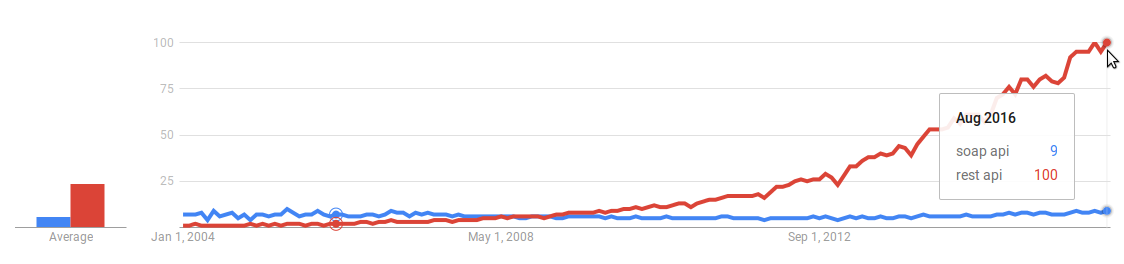
\includegraphics[height=2.5cm]{../figures/restvssoap2.png}
		\caption*{Fuente: Google Trends}
	\end{figure}	
}

\frame{ \frametitle{Evaluación y selección de un estilo arquitectural}
	\begin{figure}
		\centering
		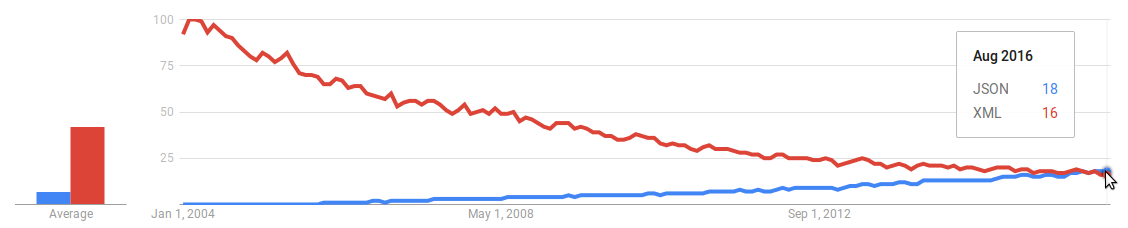
\includegraphics[height=2.5cm]{../figures/jsonvsxml.png}
		\caption*{Fuente: Google Trends}
	\end{figure}	
}

%%%%%%%%%%%%%%%%%%%%%%%%%%%%%%%%%%%%%%%%%%%%%%%%%%%%%%%%%%%%%%%%%%%%%%%%%%%%%%%%%%%%%%%%%%%%%%%%%%%%%%%%%%%%%%%%%%%%%%%%
%%%%%%%%%%%%%%%%%%%%%%%%%%%%%%%%%%%%%%%%%%%%%%%%% OBJETIVO #3 %%%%%%%%%%%%%%%%%%%%%%%%%%%%%%%%%%%%%%%%%%%%%%%%%%%%%%%%%%
%%%%%%%%%%%%%%%%%%%%%%%%%%%%%%%%%%%%%%%%%%%%%%%%%%%%%%%%%%%%%%%%%%%%%%%%%%%%%%%%%%%%%%%%%%%%%%%%%%%%%%%%%%%%%%%%%%%%%%%%

\subsection{Realizar una ejemplificación del framework. (Objetivo \#3)}

\frame{ \frametitle{Framework}
	\begin{figure}
		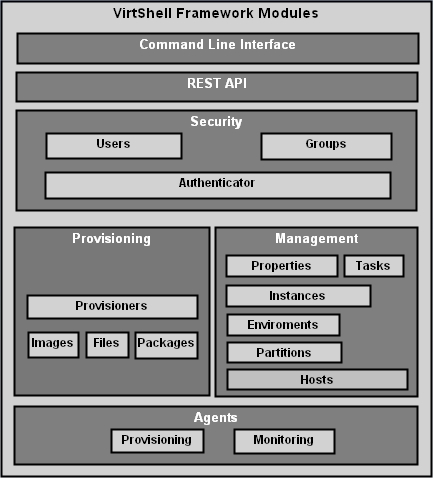
\includegraphics[width = 0.5\textwidth]{../../architecture/v1/diagrams/framework}
	\end{figure}
}

\frame{ \frametitle{Características del Framework}
	\begin{itemize}
		\item Programable
		\item Repetible
		\item Modular
		\item Seguro
		\item Extensible
		\item Inyección de dependencias virtuales
		\item Interoperable
	\end{itemize}
}

\frame{ \frametitle{Vista de componentes}
	\begin{figure}
		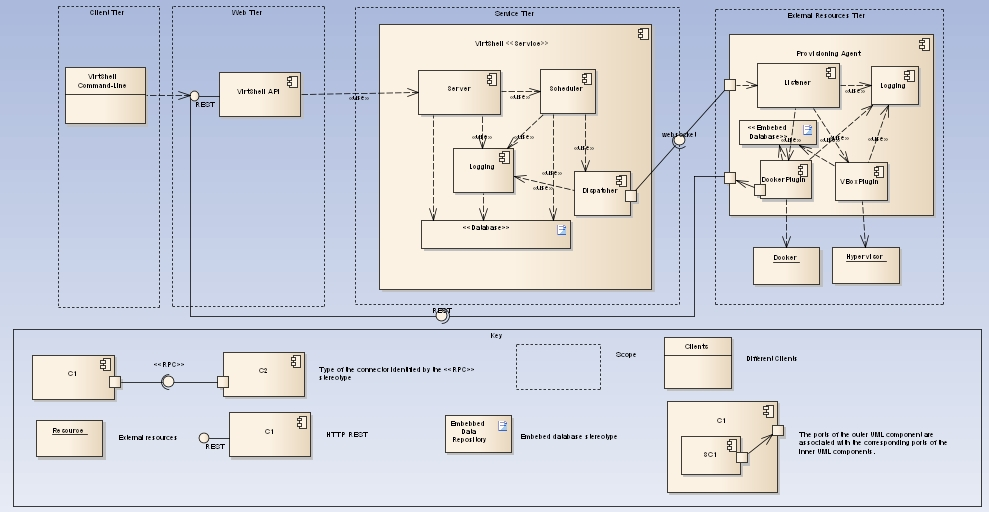
\includegraphics[height=6.4cm]{../../architecture/v1/diagrams/components.jpg}
	\end{figure}
}

\frame{ \frametitle{Vista de deployment}
	\begin{center}
		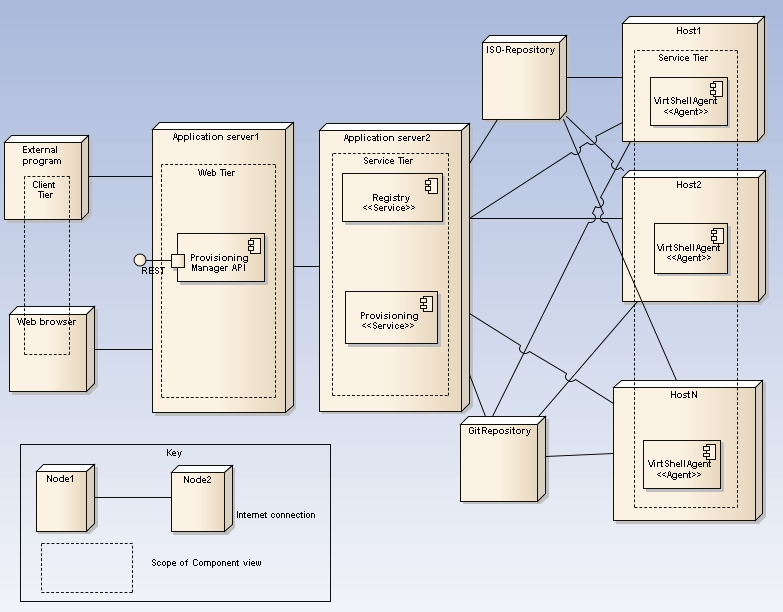
\includegraphics[height=6.4cm]{../../architecture/v1/diagrams/deployment.jpg}
	\end{center}
}

\section{Flujo de aprovisionamiento}
	\frame{ \frametitle{Flujo de aprovisionamiento}
	\begin{figure}
		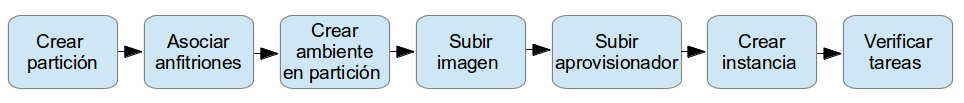
\includegraphics[width = 0.9\textwidth]{../figures/general_workflow_provisioning}
	\end{figure}
}

\frame{ \frametitle{Particiones y Anfitriones}
	\begin{figure}
		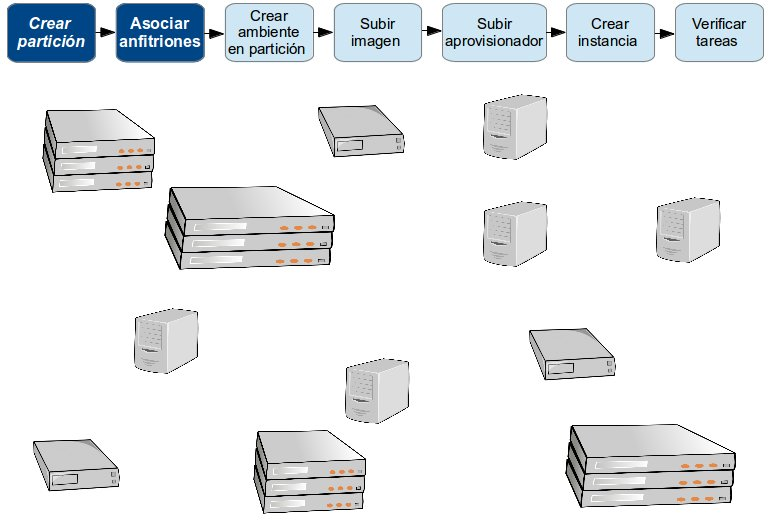
\includegraphics[width = 0.8\textwidth]{../figures/partitions_and_hosts}
	\end{figure}
}

\frame{ \frametitle{Particiones y Anfitriones}
	\begin{figure}
		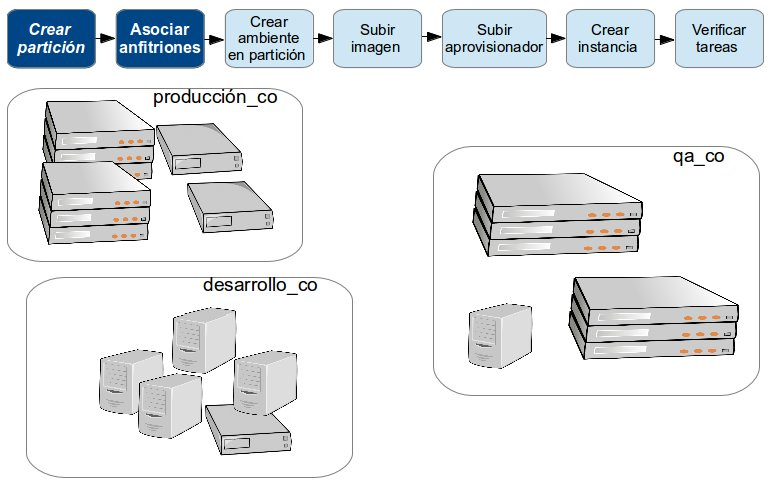
\includegraphics[width = 0.8\textwidth]{../figures/partitions_and_hosts2}
	\end{figure}
}

\begin{frame}[fragile]
	\frametitle{Creación de una partición (Ejemplo)}
	\begin{lstlisting}[language=Bash,basicstyle=\ttfamily\scriptsize,keywordstyle=\color{blue}]
	curl -X POST http://virtshellsrv:80/partitions/ 
	    -d "{\"name\":\"development_co\",
	         \"description\":\"Collection of servers oriented to development team in Colombia.\"}" 
	    -H "accept:application/json" | jq .
	\end{lstlisting}
\end{frame}

\begin{frame}[fragile]
	\frametitle{Asociación de un anfitrión a una partición (Ejemplo)}
	\begin{lstlisting}[language=Bash,basicstyle=\ttfamily\scriptsize,keywordstyle=\color{blue}]
	curl -X POST http://virtshellsrv:80/hosts/ 
	    -d "{\"name\": \"host-server-01\", 
	         \"os\": \"ubuntu-14.04.4-amd64\", 
	         \"memory\": \"2GB\", 
	         \"partition\":\"development_co\", 
	         \"type\": \"GeneralPurpose\", 
	         \"local_ipv4\": \"192.168.56.101\", 
	         \"drivers\": [\"docker\", \"lxc\"]}" 
	    -H "accept:application/json" | jq .
	\end{lstlisting}
\end{frame}

\frame{ \frametitle{Ambientes de trabajo}
	\begin{figure}
		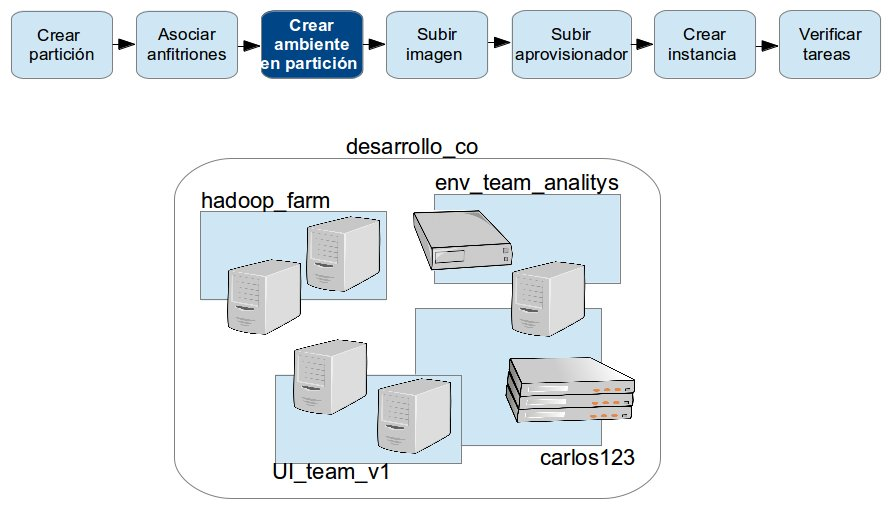
\includegraphics[width = 0.8\textwidth]{../figures/enviroments}
	\end{figure}
}

\begin{frame}[fragile]
	\frametitle{Ambientes de trabajo (Ejemplo)}
	\begin{lstlisting}[language=Bash,basicstyle=\ttfamily\scriptsize,keywordstyle=\color{blue}]
	curl -X POST http://virtshellsrv:80/enviroments/ 
	    -d "{\"name\":\"development\",
	         \"description\":\"Development enviroment\", 
	         \"partition\": \"development_co\", 
	         \"users\": [{\"login\": \"development_user\"}, 
	                     {\"login\": \"guest\"}]}" 
	    -H "accept:application/json" | jq .
	\end{lstlisting}
\end{frame}

\frame{ \frametitle{Imágenes}
	\setbeamercolor{block title}{fg=white,bg=blue!75!black}
	\begin{block}{De dos Tipos}
		\begin{itemize}
			\item ISO
			\item Templates
		\end{itemize}
	\end{block}
}

\frame{ \frametitle{Imágenes (ISO)}
	\url{https://github.com/CALlanoR/ubuntu-unattended}
}

\begin{frame}[fragile]
	\frametitle{Imágenes (ISO)}
	\begin{lstlisting}[language=Bash,basicstyle=\ttfamily\scriptsize,keywordstyle=\color{blue}]
		curl -sv -X PUT \
		    -H 'accept: application/json' \
		    -H "Content-Type: text/plain" \
		    -H 'X-VirtShell-Authorization: UserId:Signature' \
		    -d '{"name": "ubuntu_server_14.04.2_amd64",
		         "type": "iso",
		         "os": "ubuntu",
		         "timezone": "America/Bogota", 
		         "key": "/home/callanor/.ssh/id_rsa.pub",
		         "preseed_url": "https://<host>:<port>/api/virtshell/v1/files/seeds/seed_ubuntu14-04.txt",
		     "download_url": "http://releases.ubuntu.com/raring/ubuntu-14.04-server-amd64.iso"}' \
		   'http://virtshellsrv:8080/api/virtshell/v1/image' | jq .
	\end{lstlisting}
\end{frame}

\frame{ \frametitle{Imágenes (Template)}
	\begin{figure}
		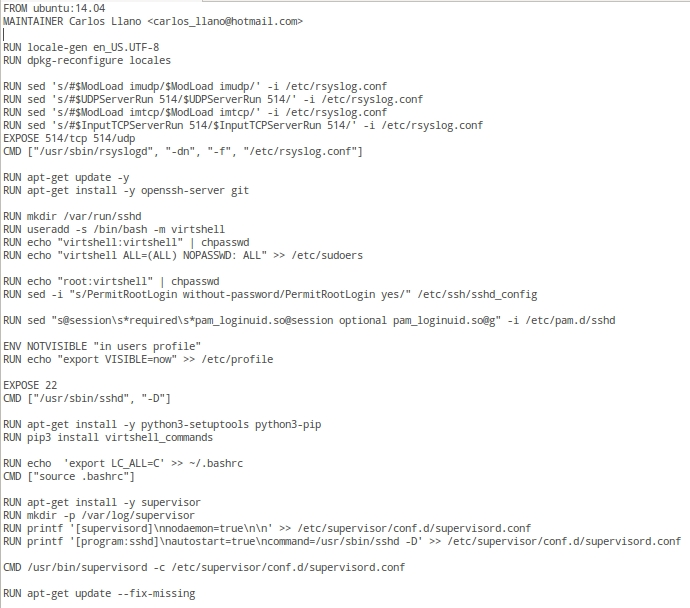
\includegraphics[width = 0.67\textwidth]{../figures/dockerfile.jpg}
	\end{figure}
}

\begin{frame}[fragile]
	\frametitle{Primero el archivo (Ejemplo - Template)}
	\begin{lstlisting}[language=Bash,basicstyle=\ttfamily\scriptsize,keywordstyle=\color{blue}]
		curl -sv -X POST \ 
		    -H 'accept: application/json' 
		    -H "Content-Type: multipart/form-data" 
		    -F "permissions=xwrxwrxwr" 
		    -F "file=@/home/callanor/Documents/Tesis/Repositories/VirtShell/virtshell_server/tests/files/dockerfile_ubuntu_server_14.04" 
		    http://virtshellsrv:80/files/  | jq .
	\end{lstlisting}
\end{frame}

\begin{frame}[fragile]
	\frametitle{Luego la imágen (Ejemplo - Template)}
	\begin{lstlisting}[language=Bash,basicstyle=\ttfamily\scriptsize,keywordstyle=\color{blue}]
		curl -sv -X POST http://virtshellsrv:80/images/ 
		    -d "{\"name\":\"ubuntu_server_14.04_amd64\",
		         \"type\":\"docker-container\",
		         \"container_resource\":\"http://192.168.56.103/file/dockerfile_ubuntu_server_14.04\"}" 
		    -H 'accept: application/json' | jq .
	\end{lstlisting}
\end{frame}


\frame{ \frametitle{Aprovisionadores (BASH Puro)}
	\url{https://github.com/CALlanoR/VirtShell_Provisioner_Simple_WebSite_Example}
}

\frame{ \frametitle{Aprovisionadores (BASH + VirtShell Commands)}
	\url{https://github.com/CALlanoR/VirtShell_Generic_Provisioner_Simple_WebSite_Example}
}

\frame{ \frametitle{Tipos de instancias}
	\setbeamercolor{block title}{fg=white,bg=blue!75!black}
	\begin{block}{Tres Tipos}
		\begin{itemize}
			\item VirtualBox
			\item Docker
			\item LXC
			\item Amazon (Under Construction...)
		\end{itemize}
	\end{block}
}

\begin{frame}[fragile]
	\frametitle{Creación de una instancia (Ejemplo)}
	\begin{lstlisting}[language=Bash,basicstyle=\ttfamily\scriptsize,keywordstyle=\color{blue}]
		curl -X POST http://virtshellsrv:80/instances/ 
		    -d "{\"name\": \"website2\", 
		         \"memory\": 1024, 
		         \"cpus\": 1, 
		         \"hdsize\": \"2GB\", 
		         \"description\": \"WebServer\", 
		         \"enviroment\": \"development\", 
		         \"provisioner\": \"generic_simple_web_site\", 
		         \"host_type\": \"GeneralPurpose\", 
		         \"driver\": \"docker\"}" 
		    -H "accept:application/json" | jq .
	\end{lstlisting}
\end{frame}

\frame{ \frametitle{Chequeo de tareas}
}


\begin{frame}[fragile]
	\frametitle{Consultar una tarea (Ejemplo)}
	\begin{lstlisting}[language=Bash,basicstyle=\ttfamily\scriptsize,keywordstyle=\color{blue}]
		curl -s http://192.168.56.103:80/tasks/b9bc6d72-cf78-4c92-bc34-c06809d4d52b | jq .
	\end{lstlisting}
\end{frame}



\frame{ \frametitle{Demo}
	\begin{figure}
		
\includegraphics[width = 0.2\textwidth]{../figures/demo.jpg}
	\end{figure}
}

%%%%%%%%%%%%%%%%%%%%%%%%%%%%%%%%%%%%%%%%%%%%%%%%%%%%%%%%%%%%%%%%%%%%%%%%%%%%%%%%%%%%%%%%%%%%%%%%%%%%%%%%%%%%%%%%%%%%%%%%
%%%%%%%%%%%%%%%%%%%%%%%%%%%%%%%%%%%%%%%%%%%% PRUEBAS Y RESULTADOS %%%%%%%%%%%%%%%%%%%%%%%%%%%%%%%%%%%%%%%%%%%%%%%%%%%%%%
%%%%%%%%%%%%%%%%%%%%%%%%%%%%%%%%%%%%%%%%%%%%%%%%%%%%%%%%%%%%%%%%%%%%%%%%%%%%%%%%%%%%%%%%%%%%%%%%%%%%%%%%%%%%%%%%%%%%%%%%

\section{Experiencia y Evaluación}

\frame{ \frametitle{Experiencia y Evaluación}
En las pruebas realizadas VirtShell demostró que parece ser una herramienta útil para aprovisionar software de manera sencilla y fiable.\\
\vspace{0.5cm}
La experiencia adquirida con la primera versión es la siguiente:
\begin{itemize}
\item \emph{VirtShell funciona}.
\item \emph{Aprovisionar ambientes virtuales via web usando scripts escritos en el lenguaje que prefiera si es posible}.
\item \emph{El aprovisionamiento de máquinas virtuales o contenedores es prácticamente el mismo}.
\end{itemize}
}

\frame{ \frametitle{Experiencia y Evaluación}
La primera versión de VirtShell fue desarrollada en el lenguaje Python (versión 3) \\
\vspace{0.5cm}
Se encuentra alojada en el repositorio git: \url{https://github.com/janutechnology/VirtShell}. \\
\vspace{0.5cm}
Esta versión inicial aun no esta terminada y se encuentra en continuo desarrollo para lograr tener todas las funcionalidades funcionando. 
}

%%%%%%%%%%%%%%%%%%%%%%%%%%%%%%%%%%%%%%%%%%%%%%%%%%%%%%%%%%%%%%%%%%%%%%%%%%%%%%%%%%%%%%%%%%%%%%%%%%%%%%%%%%%%%%%%%%%%%%%%
%%%%%%%%%%%%%%%%%%%%%%%%%%%%%%%%%%%%%%%%%%%%%%% CONCLUSIONES %%%%%%%%%%%%%%%%%%%%%%%%%%%%%%%%%%%%%%%%%%%%%%%%%%%%%%%%%%%
%%%%%%%%%%%%%%%%%%%%%%%%%%%%%%%%%%%%%%%%%%%%%%%%%%%%%%%%%%%%%%%%%%%%%%%%%%%%%%%%%%%%%%%%%%%%%%%%%%%%%%%%%%%%%%%%%%%%%%%%

\section{Conclusiones}
\frame{ \frametitle{Conclusiones}
}

%%%%%%%%%%%%%%%%%%%%%%%%%%%%%%%%%%%%%%%%%%%%%%%%%%%%%%%%%%%%%%%%%%%%%%%%%%%%%%%%%%%%%%%%%%%%%%%%%%%%%%%%%%%%%%%%%%%%%%%%
%%%%%%%%%%%%%%%%%%%%%%%%%%%%%%%%%%%%%%%%%%%%%%% RECOMENDACIONES %%%%%%%%%%%%%%%%%%%%%%%%%%%%%%%%%%%%%%%%%%%%%%%%%%%%%%%%
%%%%%%%%%%%%%%%%%%%%%%%%%%%%%%%%%%%%%%%%%%%%%%%%%%%%%%%%%%%%%%%%%%%%%%%%%%%%%%%%%%%%%%%%%%%%%%%%%%%%%%%%%%%%%%%%%%%%%%%%


\section{Recomendaciones}
\frame{ \frametitle{Recomendaciones}
}

%%%%%%%%%%%%%%%%%%%%%%%%%%%%%%%%%%%%%%%%%%%%%%%%%%%%%%%%%%%%%%%%%%%%%%%%%%%%%%%%%%%%%%%%%%%%%%%%%%%%%%%%%%%%%%%%%%%%%%%%
%%%%%%%%%%%%%%%%%%%%%%%%%%%%%%%%%%%%%%%%%%%%%%%%%% PREGUNTAS %%%%%%%%%%%%%%%%%%%%%%%%%%%%%%%%%%%%%%%%%%%%%%%%%%%%%%%%%%%
%%%%%%%%%%%%%%%%%%%%%%%%%%%%%%%%%%%%%%%%%%%%%%%%%%%%%%%%%%%%%%%%%%%%%%%%%%%%%%%%%%%%%%%%%%%%%%%%%%%%%%%%%%%%%%%%%%%%%%%%

\frame{ \frametitle{Preguntas?}
	\begin{figure}
		
\includegraphics[width = 0.2\textwidth]{../figures/preguntas}
	\end{figure}
}

%%%%%%%%%%%%%%%%%%%%%%%%%%%%%%%%%%%%%%%%%%%%%%%%%%%%%%%%%%%%%%%%%%%%%%%%%%%%%%%%%%%%%%%%%%%%%%%%%%%%%%%%%%%%%%%%%%%%%%%%
%%%%%%%%%%%%%%%%%%%%%%%%%%%%%%%%%%%%%%%%%%%%%%%%%%%%%%%%%%%%%%%%%%%%%%%%%%%%%%%%%%%%%%%%%%%%%%%%%%%%%%%%%%%%%%%%%%%%%%%%
%%%%%%%%%%%%%%%%%%%%%%%%%%%%%%%%%%%%%%%%%%%%%%%%%%%%%%%%%%%%%%%%%%%%%%%%%%%%%%%%%%%%%%%%%%%%%%%%%%%%%%%%%%%%%%%%%%%%%%%%

\end{document}